\chapter{Descriptores y  Clasificadores}
\label{cap:caract}

Tal como fue mencionado en la sección~\ref{preliminares:caract} la extracción de características como parte inicial de un algoritmo de detección de peatones es un proceso que permite describir aspectos relevantes de una imagen o vídeo como por ejemplo, color, textura, movimiento, entre otros. A este conjunto de características obtenidas se le conoce como descriptores. Para obtener estos descriptores existen gran cantidad de algoritmos, es importante entonces caracterizar el descriptor utilizado para el desarrollo del proyecto. A continuación se expone una reseña de algunos de los descriptores que se utilizan para la tarea detección de peatones según \cite{dollar2012}. Luego se indicarán las razones de la utilización del Histograma de Gradientes Orientados (HOG)~\citep{dalal2005} en el desarrollo de este trabajo. Por otra parte se revisará el funcionamiento de otros descriptores en parte teórica y en base a algunos ejemplos. En particular se expondrá breves nociones sobre SURF, propuesto por \cite{Bay2006} y \textit{Haar-like features} utilizadas por una amplia variedad de autores \citep{Papageorgiou2000, viola2001, Lienhart2002}.  

Luego de la extracción de características para determinar la existencia de un peatón en una imagen es necesario realizar un proceso de clasificación es decir serán definidas dos clases: peatón y no peatón.

Los clasificadores son algoritmos que permiten identificar y asignar un elemento que es utilizado de entrada a una categoría determinada. Sin embargo, la salida de un clasificador no es necesariamente solo una etiqueta de la categoría y en muchos casos la salida de un clasificador representa un valor obtenido una operación matemática que se encuentra descrita en el diseño de cada clasificador, los orígenes de los clasificadores son muy diversos por lo cual sus resultados no siempre son comparables.

\section{Descriptores}
\label{caract:descriptores}

Dada la elección de HOG como descriptor, es importante conocer en profundidad su funcionamiento y la forma en que se generan los vectores de características que permitirán entrenar los clasificadores utilizados en el presente trabajo. A continuación una breve introducción de cada uno de los descriptores considerados. 

\subsection{Análisis de descriptores}

\subsubsection{Histograma de gradientes orientados}
\label{descriptores:hog}

\textit{Histogram of Oriented Gradients}~(HOG) en español histograma de gradientes orientados, propuesto por primera vez por \cite{dalal2005}. Es un algoritmo descriptor de características hoy utilizado ampliamente en visión por computador para problemas de detección de objetos y en particular de la detección de personas. Esta técnica permite obtener a partir de una sección de la imagen un vector de características el cual es utilizado por algoritmos de aprendizaje de máquina para realizar una clasificación.

El método tal como fue descrito por \cite{dalal2006} está basado en la evaluación de un rejilla densa de histogramas locales normalizados de las orientaciones de los gradientes de la imagen, esto por que la hipótesis planteada era que la forma y la apariencia de un objeto estaba bien representada por la distribución local de los gradientes o direcciones de los bordes. El algoritmo tiene por estructura una cadena de cinco pasos la cual permite la extracción de este tipo de  características, los que son interesantes de conocer por lo que se explican a continuación .

\begin{itemize}
\item El primer paso es opcional dentro del proceso y consiste en realizar una normalización o ecualización de toda la imagen que tiene por objeto reducir las posible influencia de los efectos producidos por la iluminación.
\item El segundo paso corresponde al cálculo de los gradientes lo que permite describir los bordes en la imagen y también obtener información sobre la textura. Para esto se utiliza el canal de color dominante lo que permite mantener el color lo más invariante posible.
\item En el tercer paso realiza un división de la imagen en pequeños pedazos llamados \textit{``cells''} (celda) y para cada celda se calcula un histograma de gradientes local. La combinación de la información obtenida de estos histogramas locales forma el``histograma de orientación'' básico. Este método esta inspirado en el mismo tipo de características que el utilizado en SIFT \citep{Lowe2004}
\item El cuarto paso realiza una normalización, tomando un grupo de celdas al que se denomina ``bloques'' toma un valor acumulado de los histogramas locales y el resultado se utiliza para normalizar cada celda en el bloque este bloque normaliza es que se conoce como histograma de gradiente orientado.
\item Finalmente los descriptores HOG obtenidos de todos los bloques son combinados en un vector de características que se utilizan con el clasificador.
\end{itemize}

\begin{figure}[tp]
  \centering
  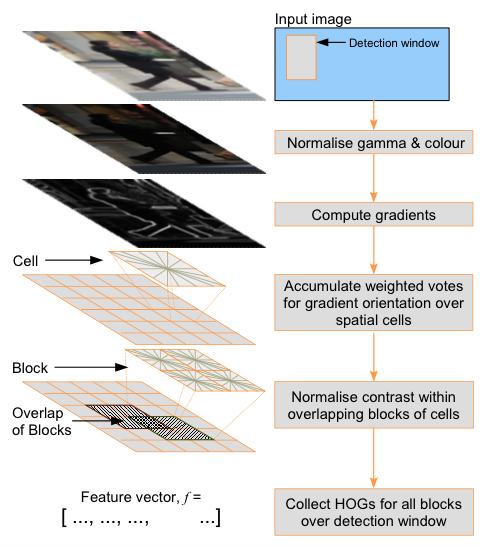
\includegraphics[scale=.6]{images/hogprocess}
  \caption{\em Estructura del proceso general de extracción de características utilizando el algoritmo de extracción HOG. Obtenido de \cite{dalal2006}}  
  \label{fig:hogscheme}
\end{figure}

\subsubsection{\textit{Scale-invariant feature transform} (SIFT)}

SIFT es un algoritmo descriptor de características utilizado en visión por computador para detectar y describir características locales de una imagen, este algoritmo fue publicado por \cite{lowe1999object}. Los algoritmos que preceden a SIFT en general se basan en la detección de esquinas ya que de esta forma las características permanecen invariante a la rotación. El principal aporte de SIFT fue que las características además permanecen invariantes en el escalado por lo que permite realizar detecciones de objetos en tamaños diferentes.

El algoritmo SIFT considera cinco etapas generales que se exponen a continuación brevemente:

\begin{itemize}
\item Detección de extremos. En esta etapa se aplica una diferencia Gaussianas en busca de máximos locales de la diferencia.
\item Localización de puntos de interés. Utilizando una expansión de serie de Taylor se localiza cada punto de interés y descarta los puntos que tengan valores inferiores a un umbral determinado. Además utilizando una matriz hessiana calcula las curvaturas principales de manera que los autovalores de la matriz no difieran en mas un orden de magnitud, eliminando así los bordes.
\item Asignación de orientación. Se calcula la magnitud y dirección del gradiente en los puntos vecinos al punto de interés generando un histograma, el punto con mayor magnitud determina la dirección del punto de interés.
\item Descripción del punto de interés. En esta etapa para cada punto de interés se define una vecindad de 16x16px la cual se divide en sub-bloques de 4x4px generando para cada unos de ellos un histograma de orientaciones. Los valores obtenidos de los histogramas son concatenados constituyendo el descriptor del punto de interés.
\item Correspondencia de puntos. Finalmente se realiza una búsqueda espacial de proximidad para relacionar los puntos de interés. Esto permite determinar que puntos de interés describen un mismo objeto. Para evitar el ruido que se pueda producir se calcula la razón entre las distancias de los dos putos mas cercanos y se filtra con un umbral determinado.
\end{itemize}

\subsubsection{\textit{Speeded Up Robust Features} (SURF)}

SURF fue presentado por primera vez por \cite{Bay2006}, este tipo de extractor de características está inspirado en \textit{Scale-invariant feature transform} (SIFT) \citep{Lowe2004}, es un descriptor orientado a la búsqueda de puntos de interés, para realizar esto se realiza una replicación de la imagen en forma piramidal gaussiana o laplaciana con el fin de obtener un efecto borroso llamado \textit{scale-space}, el cual permite obtener puntos de interés que se logran mantener invariantes al variar su escala. 

El principal aporte de SURF es que con el cambio de esquema realizado respecto de SIFT puede mejorar la velocidad de cómputo manteniendo en teoría la calidad de los puntos de interés. El cambio de esquema tiene relación principalmente con que el cálculo con gaussianas realizado en SIFT es reemplazado por aproximaciones cuadradas en SURF. Un ejemplo de los operadores utilizados se muestra en \ref{fig:gaussians}, lo que al realizar la convolución resulta mucho más rápido. Para la búsqueda de los puntos de interés se utiliza un detector de \textit{Binary Large Objects} (BLOB) basado en la matriz Hessiana nombrado \textit{Fast Hessian Detector}.

\begin{figure}[htc]
  \centering
  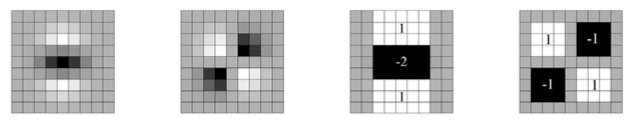
\includegraphics[scale=.6]{images/gaussian}
  \caption{\em Ejemplos de la aproximación de los gaussianas (izquierda) en cuadrados (derecha), los valores grises son cero. Imagen obtenida de \cite{Bay2006} }  
  \label{fig:gaussians}
\end{figure}

Solo para entender mejor el proceso de SURF dentro de la documentación de MATLAB es posible encontrar un ejemplo de  funcionamiento de su funcionamiento (\ref{fig:surfbox}~y~\ref{fig:surfmatching}) el cual resulta muy claro para entender lo antes expuesto. En el ejemplo se muestra un algoritmo para encontrar un objeto especifico basado en puntos clave que se corresponden entre la imagen original y la de referencia (\ref{fig:surfmatching}).

\begin{figure}[H]
  \centering
  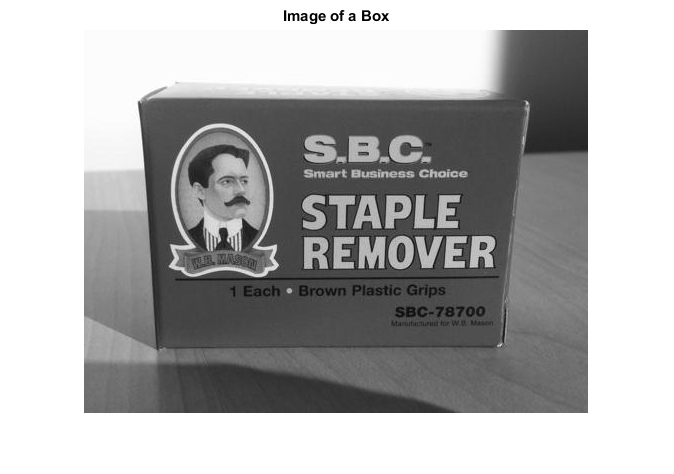
\includegraphics[scale=.4]{images/surfbox}
  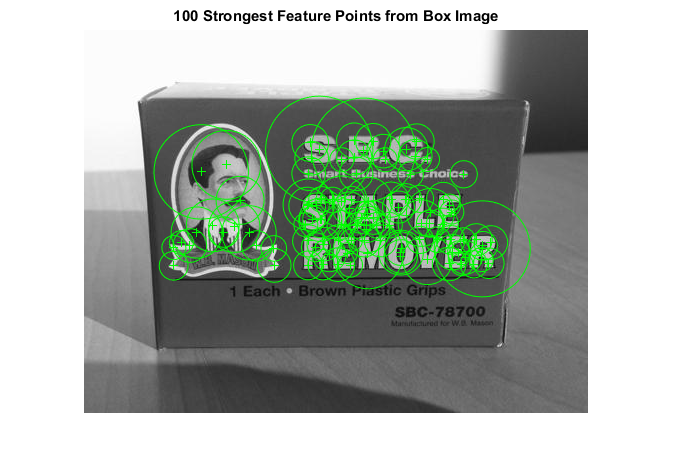
\includegraphics[scale=.4]{images/surfedbox}
  \caption{\em En la imagen, a la izquierda se observa el objeto a detectar, a la derecha el resultado obtenido luego de utilizar el detector \textit{Fast Hessian Detector} como los mostrados en la fig~\ref{fig:gaussians}. Imágenes obtenidas de \cite{matlab2014} }   \label{fig:surfbox}
\end{figure}

\begin{figure}[H]
  \centering
  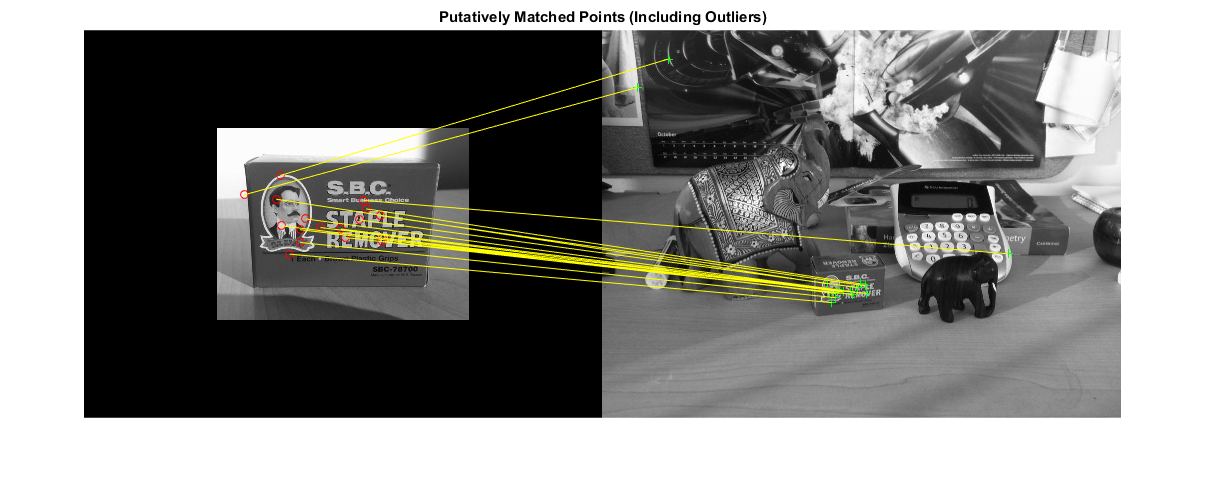
\includegraphics[scale=.4]{images/surfmatching}
  \caption{\em En la imagen. Con los puntos de interés seleccionados se realiza el proceso de búsqueda o \textit{matching}. Imágenes obtenidas de \cite{matlab2014} }   
\label{fig:surfmatching}
\end{figure}

\subsubsection{\textit{Haar-like Features}}

La extracción de características de este tipo está orientado a buscar en la imagen la presencia o ausencia de ciertas características en la imagen, como bordes o cambios de textura. En específico \textit{Haar-like Features} considera regiones rectangulares adyacentes en alguna parte de la imagen y calcula la diferencia entre las suma de las intensidades de cada píxel.

\begin{figure}[htc]
  \centering
  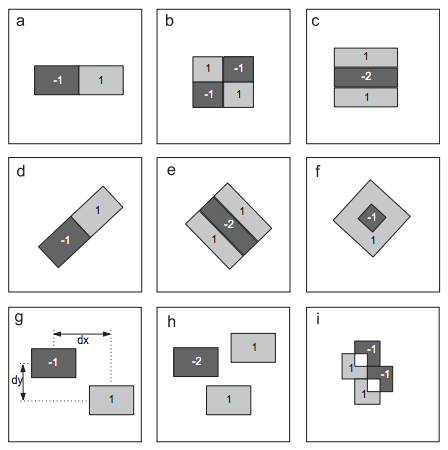
\includegraphics[scale=.3]{images/haarlike}
  \caption{\em Ejemplos \textit{Haar-like Features}. Obtenido de \cite{Pavani2010} }  
  \label{fig:haar}
\end{figure}

\section{Selección del descriptor y proceso de \\extracción de características}
\label{caract:seleccion}

Una vez revisada la información acerca de los descriptores que posiblemente se utilizarían es necesario realizar la selección del descriptor y mencionar las razones para su elección, además el proceso a través del cual se realizó la extracción de características.

\subsection{Selección del descriptor de características}

Se mencionó al inicio de este capítulo (\ref{cap:caract}) y en la sección~\ref{caract:descriptores} un adelanto del resultado sobre el descriptor que finalmente sería escogido para la realización del análisis comparativo. Aquí se ilustran las razones para su elección.

``HOG...es uno de los de los descriptores de características más comúnmente utilizado para la detección de peatones, dada su gran capacidad para describir objetos.'' \citep{Zheng2012}, de esta forma comienzan Zheng y Chen a describir HOG en \textit{``A review on vision-based pedestrian detection''}. HOG es un descriptor realmente popular que se encuentra referenciado en prácticamente cualquier trabajo del área, lo que trae consigo una amplia cantidad de información sobre este. A continuación se enuncian las razones más importante de la elección de HOG.

\begin{itemize}
\item Es un descriptor de características ampliamente referenciado, por lo que hay mucha información sobre él.
\item Se han realizado muchas aplicaciones utilizando HOG, por lo que el impacto de una posible mejoría es mayor.
\item Posee una implementación en OpenCV que es sencilla de utilizar.
\item Dado el grado de importancia conferido tiene respaldo para ser bueno como elemento para realizar pruebas.
\end{itemize}

Algunos de los aspectos negativos de esta elección es la poca variabilidad en cuanto a descriptores, sin embargo esta elección se realizó dada la prioridad otorgada a la evaluación en diferentes escalas, lo que será explicada más adelante.

\subsection{Proceso de extracción de características}
\label{caract:extraccion}

Previo al proceso mismo de extracción de características fue necesario realizar la normalización del conjunto de datos de peatones INRIA de manera que el resultado fuera directamente comparable, para realizar esto se tomaron en cuenta las siguientes consideraciones.

\begin{itemize}
\item Para facilitar la comparación final cada peatón objeto de la detección debe encontrarse en el centro de la imagen. (Esto se cumple por defecto para del conjunto de entrenamiento, mas no para el conjunto de pruebas). 

\item Se considerará en la detección toda la vecindad inmediata del peatón, es decir al comenzar la detección la ventana de clasificación se encontrará apenas fuera por la parte superior e izquierda y al finalizar se encontrará apenas fuera por la parte inferior y derecha.

\item Se considerará que el peatón se encuentra certeramente donde indican las anotaciones, aún cuando existe la certeza de que esto no es perfecto ya que en efecto hay un peatón en cada una de las anotaciones, sin embargo, no está totalmente centrado.

\item Con el fin de analizar la variación de la sensibilidad espacial a diferentes escalas, la evaluación será realizada en cuatro escalas diferentes por lo que es necesario ampliar o reducir cada imagen según sea necesario. 
\end{itemize}

%***DQ El proceso de extracción de características es directo, ya que la implementación utilizada de HOG se puede encontrar dentro de la biblioteca OpenCV y esta implementación posee la función \textit{getDescriptors} la cual recibe como entrada la imagen y entrega el valor del vector de características HOG estos vectores son recolectados en una matriz de características que luego será utilizada para el entrenamiento de los clasificadores.

En la biblioteca de visión por computador OpenCV se encuentran implementados algunas técnicas de extracción de características entre estos se encuentra HOG, esta implementación fue realizada basándose en lo descrito en el trabajo de \cite{dalal2006}. Por estas razones no es necesario utilizar un implementación propia. Las funciones implementadas reciben como entrada la imagen y entregan como resultado el vector de características.


\begin{figure}[htc]
  \centering
  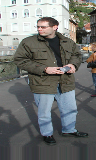
\includegraphics[scale=.6]{images/train1}
  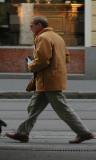
\includegraphics[scale=.6]{images/train2}
  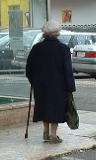
\includegraphics[scale=.6]{images/train3}
  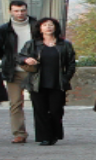
\includegraphics[scale=.6]{images/train4}
  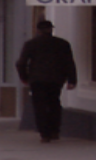
\includegraphics[scale=.6]{images/train5}\\
  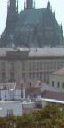
\includegraphics[scale=.9]{images/neg1}
  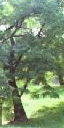
\includegraphics[scale=.9]{images/neg2}
  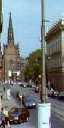
\includegraphics[scale=.9]{images/neg3}
  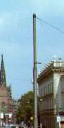
\includegraphics[scale=.9]{images/neg4}
  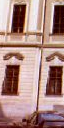
\includegraphics[scale=.9]{images/neg5}
  \caption{\em Imágenes de ejemplo obtenidas del conjunto de entrenamiento del set de datos INRIA, arriba imágenes positivas``clase peatón'', abajo imágenes negativas ´´clase no-peatón'' }  
  \label{fig:trainimgs}
\end{figure}

En la figura~\ref{fig:trainimgs} se observan ejemplos de las imágenes de conjunto de entrenamiento del set de datos INRIA de las cuales se extrae el vector de características. Con el objetivo de comparar la sensibilidad espacial a escalas diferentes se hizo necesario realizar un cambio de tamaño a las imágenes de entrenamiento del set de datos, los tamaños utilizados según la ventana de clasificación (los tamaños reales son levemente superiores para evitar problemas de borde) fueron 32x64px, 64x128px, 128x256px, 256x512px. El tamaño original de la ventana es de 64px de ancho y 128px de alto este tamaño está fijado por defecto en el set de datos, para realizar comparaciones se mantuvo la proporción 1:2, pero se amplió y redujo el tamaño de las imágenes para estudiar el comportamiento del clasificador a diferentes escalas.


\section{Clasificadores}
\label{sec:clasif}
 
Una vez determinado cuál será el descriptor de características utilizado, el siguiente paso es determinar cuáles serán los clasificadores a utilizar. En esta sección se revisarán los clasificadores estudiados, la selección, el entrenamiento y el proceso de normalización de la salida.

\subsection{Clasificadores estudiados}

\subsubsection{SVM}
\label{propuestas:svmlineal}

La implementación utilizada del SVM lineal es parte de la biblioteca OpenCV en su módulo de \textit{machine learning}. Esta implementación esta basada en la biblioteca LibSVM \citep{Chang2011}. Dentro del módulo antes mencionado no sólo es posible encontrar una implementación para SVM con un kernel lineal, sino que también para kernel polinomial, radial y sigmoidal.
Para el entrenamiento del SVM se consideraron los parámetros por defecto que se pueden observar en la figura~\ref{fig:svmparams}. Los parámetros de entrenamiento utilizados por defecto son una referencia a partir de lo descrito por \cite{dalal2006} quien a su vez indica que realizó el la búsqueda de los parámetros a partir de lo expuesto en \citep{joachims1999making}. 

\begin{figure}[htc]
  \centering
  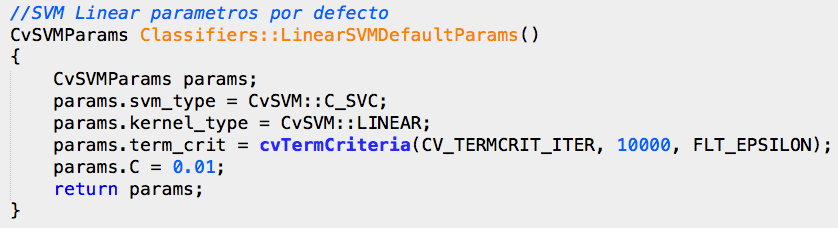
\includegraphics[scale=.5]{images/svmparams}
  \caption{\em Parámetros por defecto de SVM Lineal para la construcción de los diferentes modelos utilizados en el análisis. }  
  \label{fig:svmparams}
\end{figure}

Los modelos utilizados del clasificador SVM lineal se construyeron utilizando los vectores de características obtenidos del set de imágenes positivas para entrenamiento del set de datos INRIA y 10 recortes por imagen del set de entrenamiento con imágenes negativas también del set de datos INRIA.

\subsubsection{Adaboost}
\label{propuestas:adaboost}

Dentro del módulo de \textit{machine learning} de OpenCV es posible encontrar un sub módulo de \textit{boosting} en el cual hay algoritmos como Adaboost discreto y real, LogiBoost, y \textit{Gentle} Adaboost. Esta implementación es propia de OpenCV y está basada teóricamente en la propuestas de \cite{Hastie2005} y \cite{Friedman2000}.


\begin{figure}[htc]
  \centering
  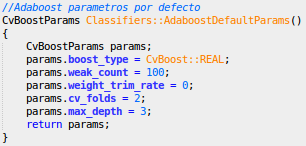
\includegraphics[scale=.6]{images/boostparams}
  \caption{\em Parámetros por defecto de Adaboost Real para la construcción de los diferentes modelos utilizados en el análisis.  }  
  \label{fig:boostparams}
\end{figure}

Al igual que para el SVM lineal se seleccionaron los parámetros por defecto, los que se pueden observar en la figura~\ref{fig:boostparams}. La selección de los parámetros fue también obtenida a partir de la literatura \citep{Zhu2006} ya que \cite{dalal2006} indica que es posible utilizar Adaboost como alternativa para realizar la clasificación. Los parámetros utilizados fueron ontenidos realizando el entrenamiento para el mismo conjuntos de datos, pero no para resolver el mismo problema por que esto podría incluir un sesgo en el estudio, esto se discutirá mas adelante.

La construcción de los modelos se realizó utilizando los mismos vectores de características (obtenidos con el algoritmo HOG) que se utilizaron para la construcción de los modelos de SVM lineal, con el fin de evitar diferencias y realizar una mejor comparación.

\section{Selección de clasificadores y entrenamiento}
\label{clasificadores:seleccion}

La selección de clasificadores fue basándose en la investigación teórica sin embargo, es conveniente indicar cuáles son las principales razones de seleccionar éstos y no otro tipo de clasificadores. Por otra parte, el proceso de entrenamiento fue exclusivamente tomar procesos ya implementados de OpenCV e incorporarlos en el proceso general. Sin embargo, como será explicado con más detalle en el capítulo~\ref{cap:eval} se realizó otro proceso de entrenamiento relacionado con la función utilizada para normalizar la salidas de los clasificadores.
% ***SAV la frase anterior es difícil de entender, podrías decir "como será explicado en más detalle en la sección xxx" ***DQ Revisado

\subsection{Selección de los clasificadores}
\label{subsect:seleccionclasif}

Los clasificadores finalmente seleccionados fueron \textit{Linear SVM} y \textit{Real Adaboost}. Desde el comienzo al buscar información sobre del problema de clasificación de personas, surgen como las herramientas de más mencionadas. Pero es \cite{dalal2006} quien, en concreto, indica que son las mejores alternativas para utilizar en conjunto con el descriptor HOG que el mismo desarrolla y presenta en un trabajo anterior \citep{dalal2005}. El trabajo de Dalal motiva en parte el desarrollo de este trabajo, esto es dado que la sensibilidad espacial en la vecindad del peatón es un punto no tratado dentro de su trabajo.  

Sin embargo, \cite{dalal2006} no es el primero es sugerir su utilización. Para el caso de SVM, como se mencionó anteriormente en la sección~\ref{preliminares:clasif}, el primero en proponer este tipo de clasificadores fue \cite{Papageorgiou2000}. La gran popularidad de SVM en general dentro de la investigación relacionada con \textit{machine learning} es muy alta, por lo que al trabajar con este tipo de algoritmos es posible encontrar gran cantidad de información y el impacto generado por una mejora también resulta mayor. Por el lado de Adaboost una de las primeras propuestas no fue directamente sobre el problema de detección de personas sino para detección de rostros \citep{viola2001}. Como SVM, Adaboost es muy popular dentro de los problemas de detección de personas. Para ser muy específico respecto de la amplia utilización de estos algoritmos en el \textit{review} realizado por \cite{dollar2012} fueron analizados dieciséis de los más relevantes clasificadores de personas publicados entre 2004 y 2010 dentro de los cuales siete usaban SVM lineal y siete Adaboost.

A continuación se enumeran las razones de la elección de SVM lineal y luego las razones para la elección de Adaboost.

\subsubsection{SVM lineal}

\begin{itemize}
\item Es un clasificador ampliamente utilizado en el problema de detección de personas.
\item Su velocidad respecto de otros kernels permite el desarrollo de aplicaciones en tiempo real.
\item Dada su popularidad, el impacto de una posible mejora es alto.
\item La cantidad de información existente es bastante, lo que facilita su utilización.
\item Se encuentra implementado dentro de la biblioteca OpenCV por lo que no requiere implementación propia y permite que el análisis sea fácilmente replicable.
\item Según el creador de HOG \citep{dalal2006} es el clasificador de elección.
\end{itemize}

Existen también desventajas respecto de la utilización de SVM lineal, sin embargo, el detalle de estas no supone una real desventaja respecto de otros clasificadores que no serán analizados.

\subsubsection{ Real Adaboost}

\begin{itemize}
\item Al igual que SVM es ampliamente utilizado en el problema de detección de personas.
\item Según la documentación en OpenCV es el algoritmo de \textit{boosting} idóneo para clasificación con dos categorías y señala que LogitBoost y Gentle Adabost tienen mejores resultados en problemas de regresión que de clasificación.
\item Dado que se encuentra en la biblioteca OpenCV no requiere implementación propia y permite que el análisis sea fácilmente replicable.
\end{itemize}

Una vez enumeradas las razones para su elección, el siguiente paso se refiere al proceso de entrenamiento que permite generar los modelos y a la normalización de su salida por medio de la utilización del sigmoide de \cite{Platt1999}.

\subsection{Entrenamiento de los modelos}

% ***SAV: al comienzo de la memoria se introdujo la base de datos de INRIA? ***DQ Revisado
Para el entrenamiento de los modelos se utilizaron los vectores de características obtenidos de las imágenes del conjunto de entrenamiento del set de datos INRIA. Estos vectores de características fueron acumulados en una matriz de características que es la que utiliza tanto SVM como Adaboost para realizar el entrenamiento. En la etapa de entrenamiento se generaron ocho modelos de clasificadores, cuatro correspondientes a SVM lineal y los otros cuatro correspondientes a Adaboost, esto por la diferencia en la escala mencionada en la sección~\ref{caract:extraccion} con el fin de verificar el comportamiento de la sensibilidad espacial en la variación de escalas.

% ***SAV porque con el mismo set de datos usados para entrenar y no con uno distinto? ***DQ revisado
Una vez entrenado cada modelo fue necesario evaluarlos con el mismo set de datos utilizado para entrenar. Estos resultados fueron recolectados y utilizados para realizar el entrenamiento de los parámetros del sigmoide, todo esto tal como indica \cite{Platt1999} en su trabajo.  El objetivo del entrenamiento de este sigmode es normalizar la salida de los clasificadores, de manera que puedan ser expresadas como probabilidades, ya que los valores de salida sin procesar de cada clasificador no permiten una comparación directa. El entrenamiento del sigmoide de Platt y sus resultados serán explicados en el siguiente capítulo.

\section{Conclusiones del capítulo}
\label{caract:conclusiones}

% ***SAV falta ... ***DQ revisado

En este capítulo se ha visto qué son los descriptores y los clasificadores. El descriptor corresponde un algoritmo que permite extraer características relevantes de las imágenes. Existe una gran cantidad de algoritmos que permiten la obtención de tales características, por tanto, se hacía necesario elegir el descriptor que sería utilizado para el presente trabajo dado el contexto. Se consideraron algunos descriptores, siendo seleccionado al final el Histograma de gradientes orientados, también conocido por la sigla HOG; producto de un proceso de selección que consideró distintos factores relevantes dentro del contexto del proyecto, que es utilizado comúnmente en la aplicación de detección de objetos en imágenes y que posee una implementación en la plataforma de software a utilizar (OpenCV).
Por otra parte, se tiene a los clasificadores, algoritmos que permiten identificar y asignar un elemento determinado a una categoría  o clase determinada. Dentro de los tipos de clasificadores estudiados se encuentran las máquinas de vectores de soporte (SVM) y Adaboost, siendo finalmente escogidos como clasificadores a Linear SVM y Real Adaboost, por su popularidad, la existencia de antecedentes anteriores que indican que estos clasificadores funcionan bien en combinación con el descriptor HOG y las ventajas de utilizarlos sobre OpenCV.
Finalmente, los dos tipos de clasificadores seleccionados fueron sometidos a un proceso de entrenamiento utilizando el set de datos de personas del INRIA en cuatro diferentes tamaños y se obtuvo ocho modelos (cuatro basados en SVM y cuatro basados en Adaboost). Con esto, ya se encuentran listos para realizar su trabajo de clasificación y ser evaluados. Sin embargo, también es necesario disponer los elementos con los que estos clasificadores van a trabajar para que cumplan las necesidades estipuladas para este trabajo, así como también aquellos que permitirán evaluar sus respuestas en lo que se refiere a la sensibilidad espacial, siendo esto materia del siguiente capítulo.

